{
\chapter{C Variables and their Segments}\label{code:c-to-segments}
\pagenumbering{Roman}
\begin{minted}{c}
// main.c

/* statically-allocated variables       	*/
/* this means they exist for the entire 	*/
/* execution of the program             	*/
/* They all go in the .bss section 			*/
/* since uninitalized or init to 0 			*/
static int aVariable;//$\label{lc-beg-statics}$
static int anotherVariable = 0;
int aVariable;
int anotherVariable = 0;

/* constant, so defined in .rodata		 	*/
static const double pi = 3.1415;

/* statically-allocated variables       	*/
/* They all go in the .data section, since	*/
/* they are initialized						*/
int anInitedVar = 42;
static int anotherInitedVar = 42;//$\label{lc-end-statics}$

/* Executable code, so defined in .text 	*/
int count() {
	static unsigned int theCount = 0; //also goes in .bss 
	return theCount++;
}
\end{minted}

\chapter{Mapping Produced by the Linker for BBPSim}\label{map:ld}

{\small
\begin{verbatim}
[... skipping output ...]

.das_state_vars_data
0x0000000000759a80      0x4f0
0x0000000000759a80                __das_state_vars_data_start = .
SORT(*obj/DasSrc/*.o)(.data .data.* .gnu.linkonce.d.*)
.data        0x0000000000759a80          0x0 obj/DasSrc/Common/src/APID.o

[... skipping output ...]

.data        0x0000000000759f40         0x30 [...]/src/RoutingProcessing.o
.data        0x0000000000759f70          0x0 [...]/src/StateHandler.o
0x0000000000759f70                __das_state_vars_data_end = .

.das_state_vars_bss
0x0000000000759f80  0x51b1068
0x0000000000759f80                __das_state_vars_bss_start = .
SORT(*obj/DasSrc/*.o)(.bss .bss.* COMMON)
.bss           0x0000000000759f80        0x0 obj/DasSrc/Common/src/APID.o
.bss           0x0000000000759f80        0x0 obj/DasSrc/Common/src/Crc16.o

[... skipping output ...]

.bss           0x000000000590a8e0      0x3b8 [...]/src/RoutingProcessing.o
*fill*         0x000000000590ac98        0x8 
.bss           0x000000000590aca0      0x348 [...]/src/StateHandler.o
0x000000000590afe8                __das_state_vars_bss_end = .
\end{verbatim}
}
\chapter{Sanitized List of DAS Variables}\label{das-symbol-catalog}

{\small
\begin{verbatim}
e6069e4f97d40996a8ea84bbb62eaf6b16aec786
0000000000759a80 0000000000000000 __das_state_vars_data_start
0000000000759a80 0000000000000004 m_u32DasSwTraceFilter
0000000000759aa0 0000000000000040 asTflLoadingOrder
0000000000759ae0 0000000000000020 asDidlLoadingOrder
0000000000759b00 0000000000000030 asIpclLoadingOrder
0000000000759b40 0000000000000001 m_u8PageReadCount
0000000000759b60 0000000000000054 m_u32BinaryFileSizeStatus
0000000000759bc0 0000000000000020 m_aeFileLoadStatus
0000000000759be0 0000000000000040 m_strBinaryFileList
0000000000759c20 0000000000000008 m_asExtCmdTlmSubsystem
[... skipping output ...]
0000000000759d10 0000000000000008 m_asRsVcduRxCntTlm
0000000000759d18 000000000000000c m_asFrameSyncMissCntTlm
0000000000759d24 000000000000000c m_asFrameSyncDetectCntTlm
0000000000759d30 000000000000000c m_asVcduTxCntTlm
0000000000759d3c 0000000000000008 m_asIdleFrameTxCntTlm
0000000000759d44 0000000000000008 m_asDataFrameTxCntTlm
0000000000759d4c 000000000000000c m_asPassThroughTxCntTlm
0000000000759d60 0000000000000016 m_au16CmdMsgTimeoutInMs
0000000000759d80 0000000000000020 m_sFtfcMemPool
0000000000759da0 0000000000000020 m_sGtwMemPool
0000000000759dc0 0000000000000120 m_asRfcuRffeReceiver
0000000000759ee0 0000000000000028 m_au8TimeSuitePerRate
0000000000759f08 000000000000000c m_au8C2v2RateToTimeConversion
0000000000759f20 0000000000000014 m_au8TdrsRateToTimeConversion
0000000000759f40 0000000000000030 mc_asVcidFtrList
0000000000759f70 0000000000000000 __das_state_vars_data_end
0000000000759f80 0000000000000000 __das_state_vars_bss_start
0000000000759f80 0000000000000004 m_bDasIntegrationTraceFilter
[... skipping output ...]

\end{verbatim}
}

\chapter{Symbol Cataloging Process}\label{fig:blackbox-diagram}
\begin{figure}[H]
	\centering
	\includesvg[width=\linewidth]{svg/blackbox-diagram}
	\caption{Sequential steps to include the symbol catalog in \pathmono{libBbpSim.so}}	
\end{figure}

\chapter{Stack-Copying Assembly Routine}\label{code:stk-copy-asm}

\begin{minted}{c}
void bbpsimThreadRestoreEntry() {
	asm volatile(
	 "  xor   %%r10, %%r10               \n\t" //r10 is the counter
	 "copyquadword:                      \n\t" //$\label{code:copyqword-beg}$
	 "  cmpq  %[length], %%r10           \n\t"
	 "  jnb   copyend                    \n\t"
	 "  movq  (%[other]), %%rax          \n\t"
	 "  movq  %%rax, (%[cur])            \n\t"
	 "  addq  $8, %%r10                  \n\t"
	 "  subq  $8, %[other]               \n\t"
	 "  subq  $8, %[cur]                 \n\t"
	 "  jmp   copyquadword               \n\t"
	 "copyend:                           \n\t"
	 "  movq   %[context], %%rdi         \n\t"//arg to setcontext
	 "  movq   %[sp], %%rsp              \n\t"//set stack pointer
	 "  jmpq   *%[setcontext]            \n\t"//doesn't return
	 ://outputs (none)
	 ://inputs, constraint all to registers, can't touch memory
	     [context] "r"(sc),                         //= register set
	     [sp] "r"(sc->uc_mcontext.gregs[REG_RSP]),  //= new stack pointer
	     [length] "r"(u64SizeOfCopy),               //= $\Delta_{usr}$
	     [cur] "r"(fswthread->m_pi8StartUserStack), //= current stack start
	     [other] "r"(pi8RestoreStartUserStack),     //= old stack start
	     [setcontext] "r"(&setcontext)              //= address of setcontext 
	 ://clobbered registers
	     "rax", "rdi", "r10"
	);
	
	return; //should never get here
}
\end{minted}

\chapter{Environment Saver Use Case}\label{code:env-saver-use}

\begin{minted}{c++}
eModuleStatus CFifoManager::SaveTo(CEnvironmentSaver& rclEnvSaver, void* pvArg)
{
	CFifoQueue* pclQueue = nullptr;
	for(auto itFifo : m_clFifos)
	{
		pclQueue = itFifo.second;
		rclEnvSaver.BeginBlock(RB_FIFO);
		rclEnvSaver.AddToBlock(itFifo.first); // fifo id
		rclEnvSaver.AddToBlock(pclQueue->GetMessageSize());//fifo element size
		rclEnvSaver.AddToBlock(pclQueue->GetQueueMaxLength());//fifo queue length
		//let the queue save its messages
		pclQueue->SaveTo(rclEnvSaver);
		rclEnvSaver.EndBlock();
	}
	return BBPSIM_STATUS_OK;
}
\end{minted}

\chapter{Environment Restorer Use Case}\label{code:env-restorer-use}

\begin{minted}{c++}
eModuleStatus CFifoManager::RestoreFrom(CEnvironmentRestorer& er, void* pvArg) 
{
	eModuleStatus eRet = BBPSIM_STATUS_ERROR;
	CFifoQueue* psNewFifo = nullptr;
	FifoID fifoID;
	UINT32 u32ElemSize, u32MaxQueueLength;
	
	er.QueryBlockType(RB_FIFO); //<- throws when no block of this type

	do
	{
		//read queue constructor attributes
		er.ReadFromBlock<FifoID>(&fifoID);
		er.ReadFromBlock<UINT32>(&u32ElemSize);
		er.ReadFromBlock<UINT32>(&u32MaxQueueLength);
		psNewFifo = new CFifoQueue(u32ElemSize, u32MaxQueueLength, "");
		//fill new queue with read messages
		psNewFifo->RestoreFrom(er);
		//add queue to container
		m_clFifos[fifoID] = psNewFifo;
	}
	while(er.NextBlock()); 
	
	return BBPSIM_STATUS_OK;
}  
\end{minted}

\chapter{RAM Profiling Output}\label{app:ram-profiling}
\begin{verbatim}
Command being timed: "./test.elf"
	User time (seconds): 0.77
	System time (seconds): 0.12
	Percent of CPU this job got: 100%
	Elapsed (wall clock) time (h:mm:ss or m:ss): 0:00.89
	Average shared text size (kbytes): 0
	Average unshared data size (kbytes): 0
	Average stack size (kbytes): 0
	Average total size (kbytes): 0
	Maximum resident set size (kbytes): 261248
	Average resident set size (kbytes): 0
	Major (requiring I/O) page faults: 0
	Minor (reclaiming a frame) page faults: 44449
	Voluntary context switches: 33
	Involuntary context switches: 5
	Swaps: 0
	File system inputs: 0
	File system outputs: 16
	Socket messages sent: 0
	Socket messages received: 0
	Signals delivered: 0
	Page size (bytes): 4096
	Exit status: 0
\end{verbatim}

\chapter{Valgrind Profiling Output}\label{app:valgrind-profiling}
\begin{figure}[H]
	\centering
	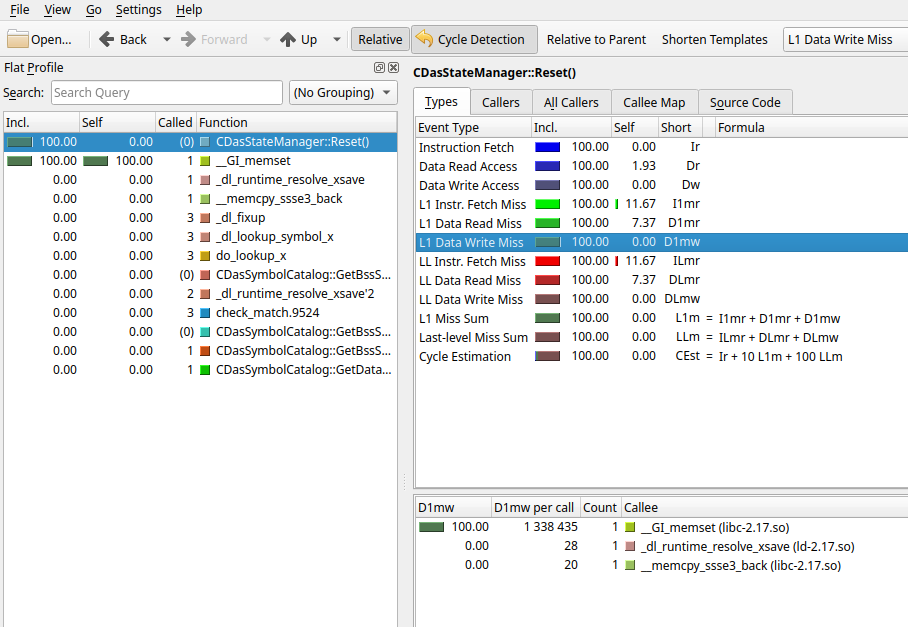
\includegraphics[width=\linewidth, keepaspectratio]{art/reset-perf.png}
\end{figure}
}